\documentclass[a4paper, oneside, 11pt]{article}
\usepackage{graphicx} % Required for inserting images

\usepackage[margin=2cm]{geometry}
\usepackage[style=ieee]{biblatex}
\addbibresource{references.bib}

\title{Human Pose Recognition for Classifying Grappling Positions}
\author{Talhaa Hussain}
\date{}
\begin{document}
\pagenumbering{roman}

\maketitle

\begin{abstract}
    Grappling is a form of unarmed combat that doesn't involve strikes (i.e. punches, kicks, knees, elbows or headbutts), and instead revolves around takedowns, ground control and submission holds. There are many variants of grappling, but generally the objectives are the same - to either pin an opponent to the ground and prevent them from moving, or to cause them to concede/submit, either through a choke/stranglehold or through a joint lock.

    Unlike striking, grappling is much more complex due to the range of techniques, positions, submissions and holds available. This can make identifying positions and techniques (either when learning or officiating a grappling match) quite difficult. This project aims to use machine learning and computer vision to identify different positions in grappling, outline and build a solution, and provide a timeline for the development of the solution. Machine learning techniques has been shown to be capable of identifying and distinguishing different positions and patterns of the human body, such as faces, hands or posture. This report aims to propose a solution that uses human pose estimation and machine learning techniques to identify and recognise different positions in grappling.  
\end{abstract}

\vspace*{\fill}
\textit{\textbf{I certify that all material in this report which is not my own work has been identified.}}
\newpage

\tableofcontents

\newpage
\pagenumbering{arabic}

\section{Introduction}

\subsection{Motivation}

This project aims to leverage advanced computer vision techniques and machine learning to identify and classify various positions in grappling, a form of unarmed combat and class of sports that revolves around controlling an opponent. A pipeline is proposed for first identifying a pair of grapplers (combatants), isolating their joints and limbs, and passing this to a machine learning algorithm to decide what grappling position they are currently in. 

\bigskip
\noindent
I hope to show the potential practical application of computer vision and human pose estimation to the world of combat sports, with uses ranging from more traditional arts, such as Judo, to more recent developments, such as modern mixed martial arts. Potential use-cases include automated judging/refereeing, generating educational content and additional insights into the sports, or analysis of one's own performance.

\bigskip
\noindent

\subsection{Adaptations}

When this project was first conceived, the original intention was to produce a product that could distinguish between various positions across three main grappling forms (Brazilian Jiu-Jitsu, Judo and Olympic wrestling). However, after analysis of existing material and in-depth discussion with subject experts and HPE (human pose estimation) specialists, this idea has changed slightly. In order for this change to be fully explained, some context and insight into grappling must first be given.

\bigskip
\noindent
Grappling can take place standing up or on the ground. Striking is not permitted in grappling, and instead the focus is on controlling your opponent through grips, clinch-holds, takedowns, guards, pins and other controlling positions. Some forms of grappling, such as Brazilian Jiu-Jitsu, also involve submission holds - forcing an opponent to give up, or "tap out" by applying a joint lock or a stranglehold. Other grappling forms, such as Olympic wrestling, have a different objective - pinning an opponent on their back for a number of seconds, such that both shoulder blades touch the ground simultaneously. Regardless of the win condition(s), in all forms of grappling and combat, being pinned to the ground is universally considered a losing position, while pinning an opponent is considered a winning position (as this allows a player to attempt submissions with little threat).

\bigskip
\begin{figure}[h]
    \centering
    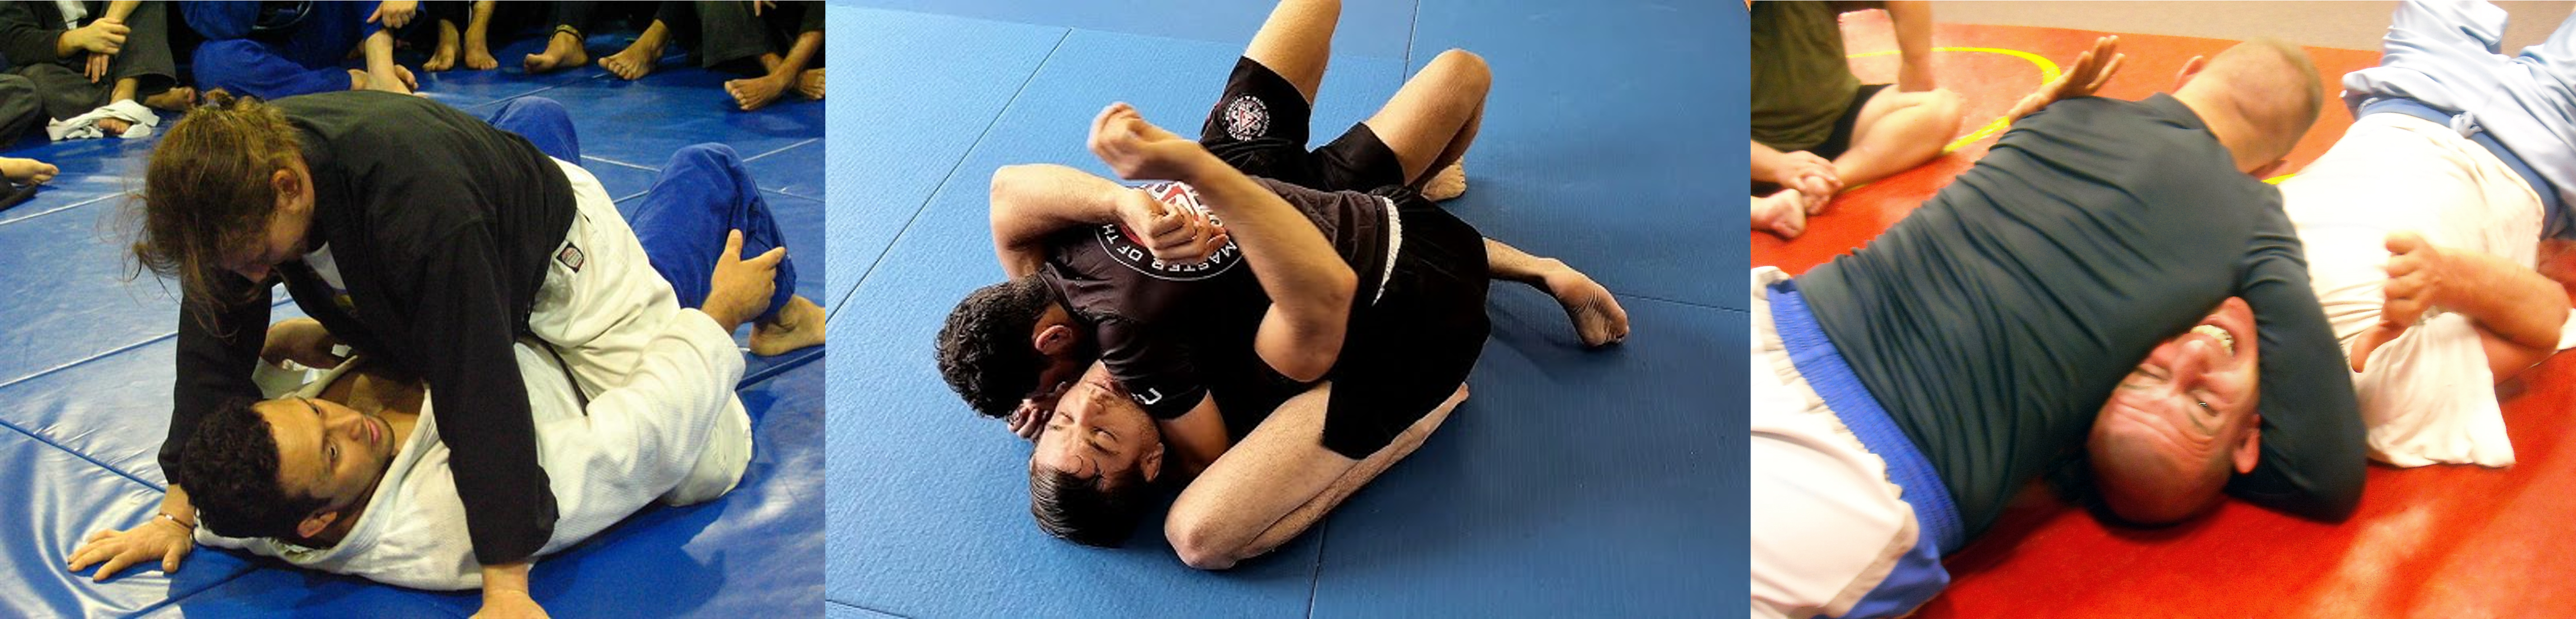
\includegraphics[scale = 0.40]{img/pins.png}
    \caption{The most common grappling pins. From left to right: mount, side control, north-south.}
    \label{fig:grapplingpins}
\end{figure}

\bigskip
\noindent
There are several forms of pinning common to all grappling sports, the most notable three being shown above. In order to increase the feasibility of the project, the objective was adapted - rather than trying to classify many different grappling positions in a highly occluded scenario, we would aim to identify whether or not a particular position was a pin. This new objective allows the product to generalise across grappling sports much better, rather than being bound to a single paradigm (e.g. Jiu-Jitsu). As well as being much more adaptable across unified grappling, identifying pins can allow the proposed system to act as a referee in certain forms of competition, especially Judo and wrestling, where a pin is considered a win condition.

\subsection{Related Works and Existing Solutions}

Presently, there is no unified exiting solution or framework for the problem at hand. However, similar problem spaces have been explored before, most notably the work of V. Hudovernik and D. Skočaj in their 2022 paper "Video-Based Detection of Combat Positions and Automatic Scoring in Jiu-jitsu" \cite{IdentifyingBJJPositions}. This solution is fairly similar to the problem at hand, but restricts itself to Brazilian Jiu-Jitsu (BJJ), a specific grappling sport, rather than looking to generalise for all grappling systems. Nonetheless, guidance and inspiration can be drawn from the methodology proposed here, as the researchers likely had to deal with similar challenges with regards to occlusion and difficulty when classifying positions. I will be making frequent reference to these researchers, and employ architectures and techniques that are inspired by them and their work.

\section{Project Specification}

\subsection{Considerations and Challenges}

By far the largest challenge present, when applying computer vision to grappling, is the high level of occlusion in the environment. Unlike most situations where human pose estimation is typically used, grapplers tend to be very "entangled" with one another, making it difficult for a model to distinguish the individuals, identify their joints and accurately detect/predict the location of their major limbs. Previous solutions to similar problems, such as that of V. Hudovernik et al., overcame this issue by using multiple camera angles and a time series \cite{IdentifyingBJJPositions}. However, the use of multiple camera angles falls outside of the scope of this project, as this would introduce a massive amount of complexity when it comes to keeping track of the different angles, the different frames in the time series, changing angles and prioritising estimations between angles. Instead, I will make use of frame-by-frame analysis of an exchange, applying computer vision techniques on each frame in isolation to make predictions and gather data on the competitors.

\bigskip
\noindent
The close proximity of the combatants also means that the clothing worn by competitors also has a large influence over how occluded the exchange may be, from a computer vision point of view. If two competitors are engaged while wearing a Gi - a loose jacket worn in Judo, Sambo, Kudo and other grappling sports - the occlusion of the scene would be much higher, since the jacket and pants obscure their limbs and may "hide" certain keypoints and distinguishing elements (such as hands or feet). As such, I will prioritise the use of data where combatants are wearing more form-fitting clothing, such as a rashguard, short and spats, or a singlet. 

\subsection{Objectives and Success Criteria}

To be considered fully successful, the project must be able to carry out the following objectives:

\begin{enumerate}
    \item The program must be able to take a video or image input, and provide an output of the same type:
    \begin{enumerate}
        \item In the event that a video is provided, it should be split into individual frames, and frames should be concatenated once against post-processing.
        \item Video frames must be processed as image frames.
    \end{enumerate}
    \item An output (image or video) must have the following:
    \begin{enumerate}
        \item Bounding boxes around both combatants.
        \item Identified keypoints of both combatants.
        \item Text indicating whether or not a position is a pin.
        \item A confidence score on whether a position is a pin or not.
        \item Colours indicating whether or not a position is a pin or not (green for yes; red for no).
    \end{enumerate} 
    \item The program must process images and video within "reasonable time":
    \begin{enumerate}
        \item For an image, reasonable time is from 3 to 5 seconds on an Intel Xeon CPU with 2 vCPUs (virtual CPUs) and 13GB of RAM (as provided by Google Colaboratory).
        \item For a 720p, 30fps video, reasonable time is 1 second per 1 second of video footage on an NVIDIA Tesla T4 GPU with 16GB of VRAM (as provided by Google Colaboratory).
        \item Google Colaboratory will be the platform upon which this is judged.
    \end{enumerate}
    \item The program must implement two machine learning algorithms:
    \begin{enumerate}
        \item A human pose estimation (HPE) model to detect two individuals in a given image/frame, outputting:
        \begin{itemize}
            \item A bounding box for each athlete.
            \item The keypoints of each athlete (described later).
        \end{itemize}
        \item A classification model, outputting:
        \begin{itemize}
            \item A binary classification for an image, determining whether or not an athlete has pinned another athlete. 
        \end{itemize}
    \end{enumerate}
    \item The program's classifier must achieve an F1-score of 0.7 or higher.
    \item Results must be easily reproducible by a third party, specifically:
    \begin{enumerate}
        \item By providing the means to train/use any machine learning models.
        \item By clearly explaining how the dataset was obtained and adapted.
        \item By clearly providing names of any libraries or modules used.
    \end{enumerate}
\end{enumerate}

\bigskip
\noindent
The scope and evaluation of the project will be limited to the dataset (described later), as attempting to build a solution that generalises to different camera angles, elevations, colour schemes and modes, lighting conditions and number of people in a given frame/image is too large of a scope for a single project. Nonetheless, the project will be designed and implemented with generalisability in mind, acting as a proof of concept and framework for potential future projects or implementations. Other data from outside the dataset may be used for analytics, but will not be included as part of the results. Furthermore, the final product is expected to work on two combatants, and two combatants only. The product is not expected to be able to handle any different amount of people, and the binary classifier will simply not be run if this is the case.

\section{Design}
\subsection{Design Philosophies and Key Ideas}
The project will be developed in Python 3. This is because Python supports a variety of libraries that are essential to machine learning, such as NumPy (for handling arrays and matrices), Pandas (for data manipulation), OpenCV (to aid with computer vision) and PyTorch (a popular machine learning library). Python is widely used in the fields of data science and computer vision, and the libraries mentioned are well-maintained and widely used for purposes very similar to this project.

\bigskip
\noindent
The project will be developed in a Jupyter Notebook, through Google Colaboratory. The platform provides access to powerful hardware, such as GPUs and TPUs, which can be leveraged for both training and testing. Without this specialised hardware, most machine learning actions would take significantly longer, thereby increasing the impact of mistakes or missteps made during development. Jupyter Notebooks also allow the inclusion of instructions, making results easier to reproduce and code easier to follow. Additionally, Google Colab is a universally available platform, accessible through any modern browser, meaning platform dependence is not as much of an issue, and anyone can easily access and run the source code. Many of the latest computer vision models support Colab, with some even being developed heavily in Jupyter Notebooks. Finally, Colab also supports project collaboration and is widely used by contemporary data scientists and computer vision experts, making it easy to communicate ideas and draw inspiration from others.

\bigskip
\noindent
A unifying theme of this project will be modularity and a priority on interacting with secondary storage, rather than displaying images or videos. The very nature of this project necessitates a lot of interaction with images and video and while other similar projects may support live video capture, for example, from a webcam, this project will instead aim to load and save video to and from the file-system. This is because live recording and video-streaming are very performance-intensive tasks, in a project that is already quite computationally expensive. Choosing live recording and playback as a paradigm for communicating with the user may result in drops in performance. This also places a lot of dependence on the end-user and their hardware, which leads to unpredictable performance on certain devices. Following this philosophy, the machine learning models themselves will be portable, allowing the user to save, store and load them easily for later use. This will be discussed further in a later subsection.

\bigskip
\noindent
The project intends to support both video and image inputs, making predictions on either input that aim to be as accurate and consistent as possible. As a result of this, video classification will be done by simply splitting a video into individual frames, processing these frames as if they were individual images, and stitching the processed frames back together to return a video. One of the major benefits of this is that the pipeline is massively simplified, while still enjoy a large boost in usefulness and versatility. While the audio from the original video may be lost during this process, this won't have any major effect on the success of the product, as audio processing isn't handled by the algorithm.

\subsection{The Architecture}

The proposed architecture originates from a literature review conducted previously. The high-level overview (shown below) was proposed after looking at approaches taken by other researchers for similar problems. 

\bigskip
\begin{figure}[h]
    \centering
    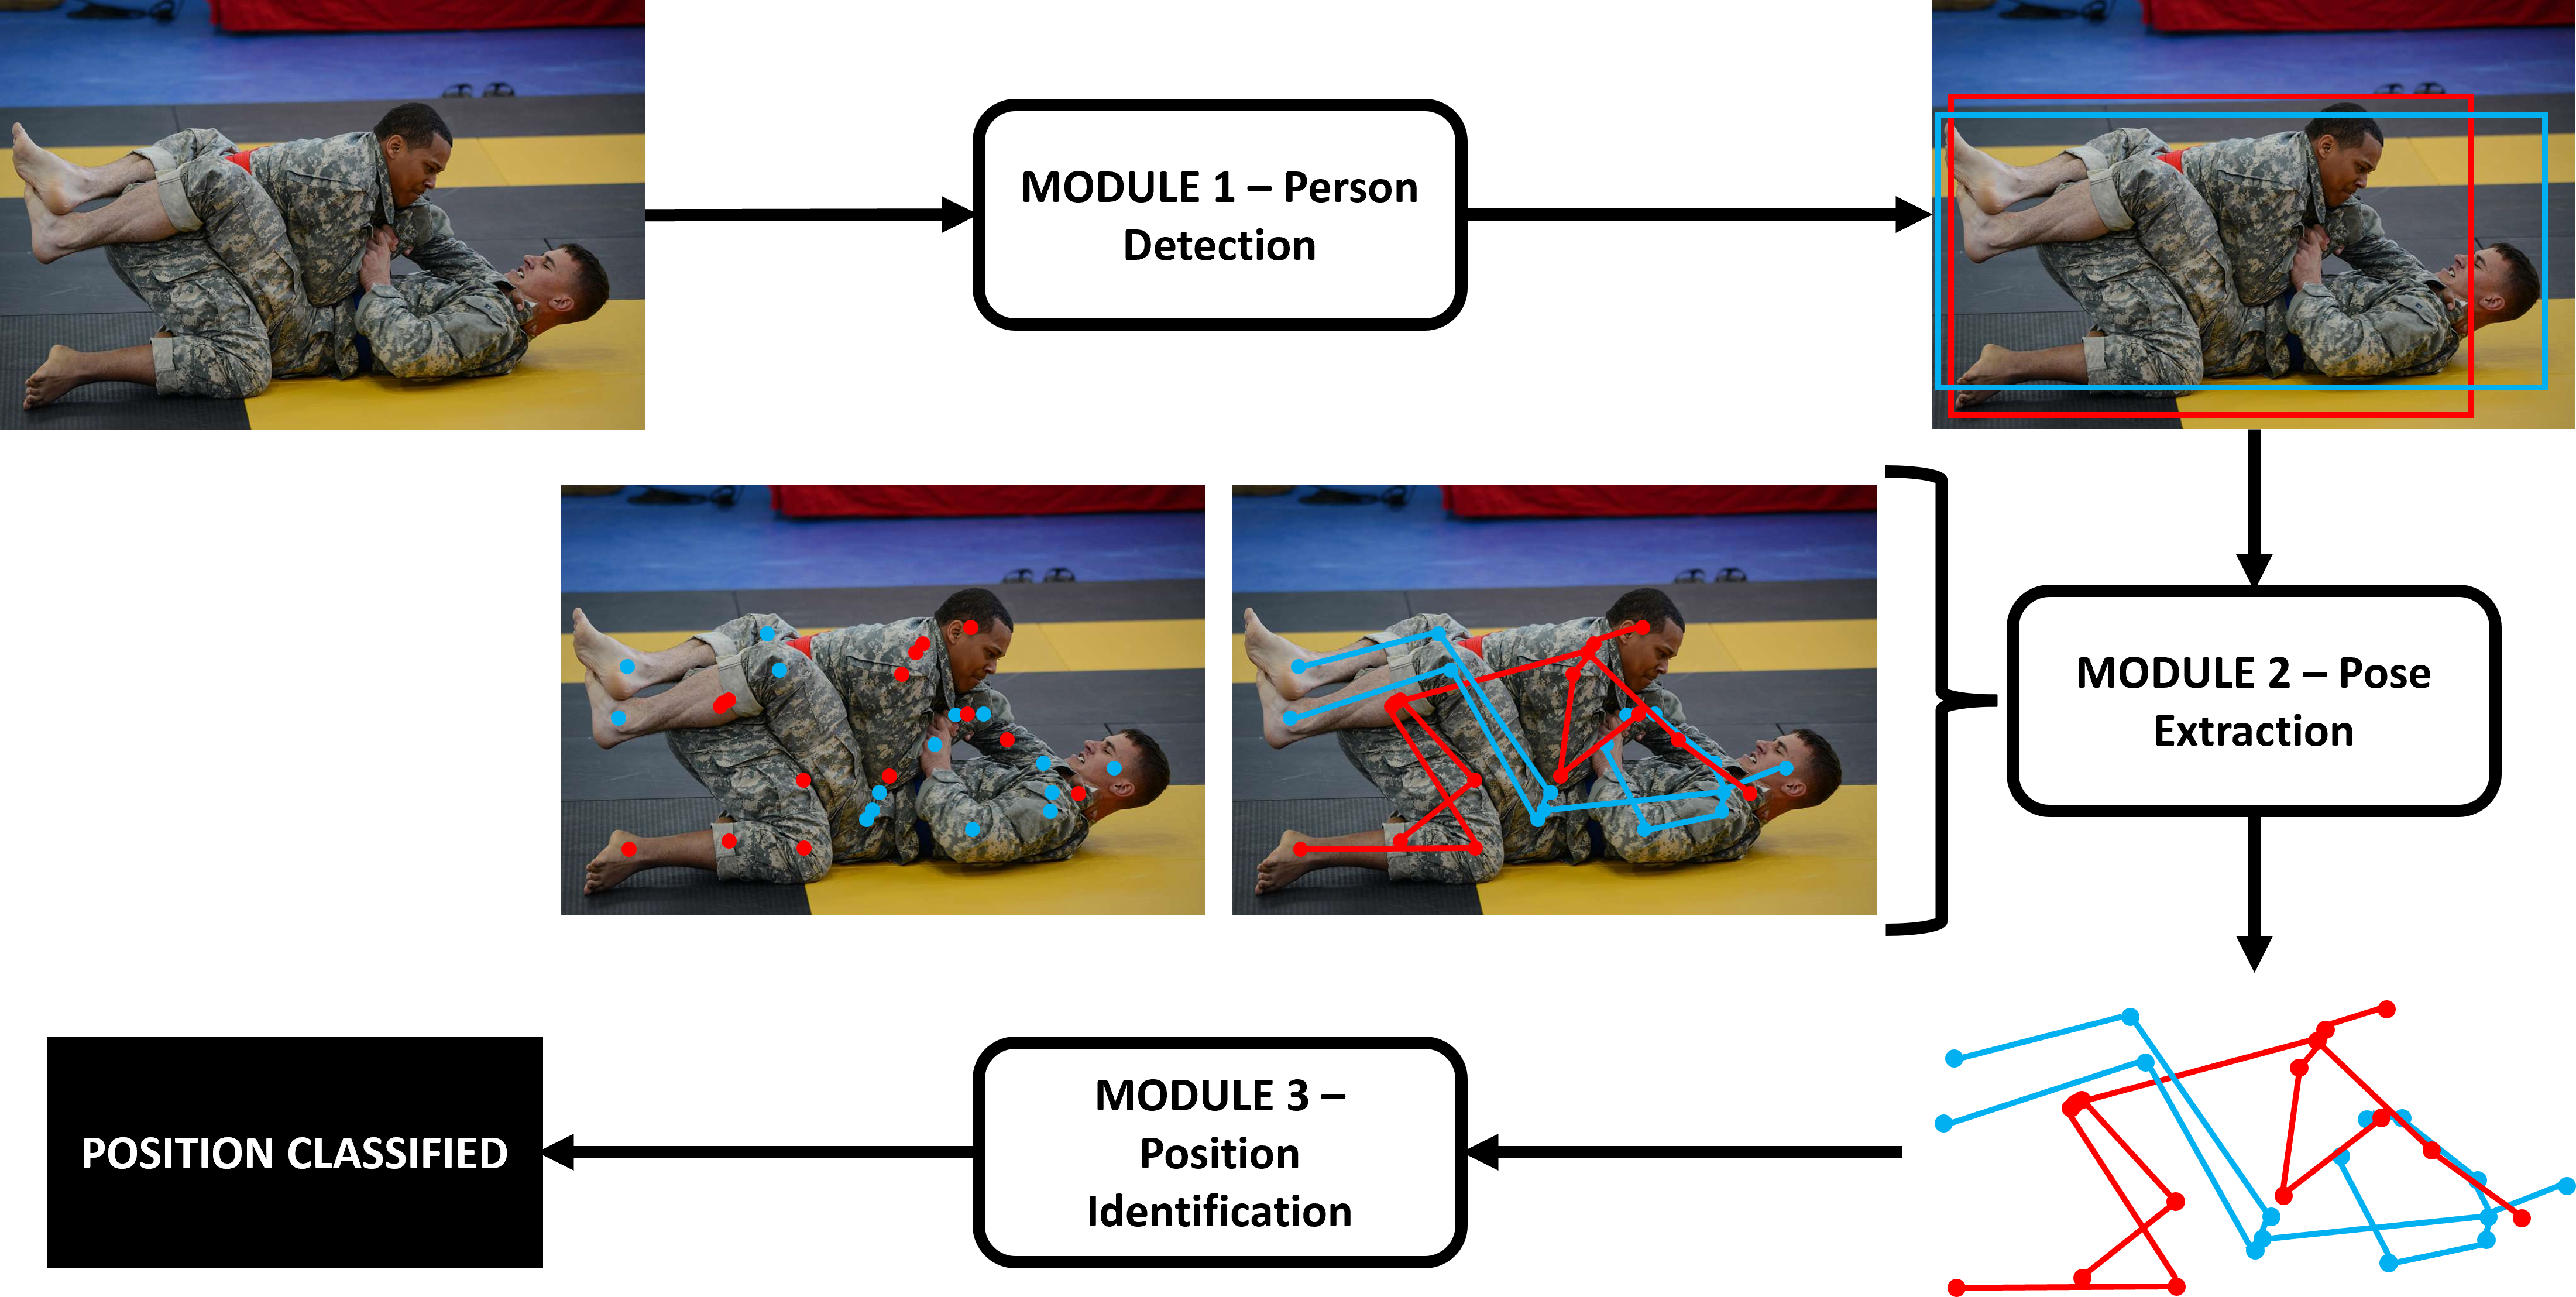
\includegraphics[scale = 0.5]{img/operations.png}
    \caption{Proposed approach pipeline}
    \label{fig:grapplingpositions}
\end{figure}

\bigskip
\noindent
Two key models are used in this architecture - a computer vision (HPE) model, for identifying individuals and extracting keypoints, and a classifier, for identifying their combat position. This two-stage approach is taken because it allows the pipeline to filter out any "noise", or unnecessary data in the background, and focus purely on the two competitors, and the coordinates of their joints. This also allows for a simplified classification model to be used, since feature extraction is carried out at an earlier stage in the pipeline. This will be discussed in more depth later in this section.

\bigskip
\noindent
This pipeline makes use of a kinematic, 2-dimensional pose estimation model, due to the relatively low overhead cost. A top-down approach is used (where individuals are identified first, using a bounding box, before identifying, aggregating and assigning keypoints) \cite{HPEGuide}. A key benefit of the top-down approach is that it works much better when there is a large amount of overlap between the individuals \cite{HPEDeepLearningMethods}, which is usually the case in combat sports. Additionally, since grappling competitions only ever take place between two competitors at once, there is a definite certainty to how many humans need to be identified in a given image/frame.

\subsection{The Dataset and Preprocessing}
For 2-D human pose estimation, the most commonly used format for kinematic (skeletal) models is the MS-COCO (Microsoft Common Objects in Context) format \cite{MSCOCO}. This format involves identifying 17 different keypoints on an individual, and recording the coordinates of these points in an $(x, y, \textit{confidence})$ format. The keypoints (in order) are shown in the figure below.

\bigskip
\begin{figure}[h]
    \centering
    \includegraphics[scale = 0.47]{img/ms-coco.png}
    \caption{Keypoints on a kinematic HPE model. Arcs are for illustrative purposes only.}
    \label{fig:keypoints}
\end{figure}

\bigskip
\noindent
Initially, I had planned to generate my own dataset, through recordings of myself and other consenting individuals grappling, splitting these videos into individual frames for training and testing. However, I was unable to find a consenting venue for recording, and had to rely on a publicly available dataset of images instead.
Such a dataset was provided by the Visual Cognitive Systems Laboratory, at the University of Ljubljana, Slovenia, licensed under Creative Commons Attribution-NonCommercial-ShareAlike 4.0 International License \cite{IdentifyingBJJPositions}. All credits go to the original owners.

\bigskip
\noindent
The dataset consisted of 120'279 images, with a single JSON file, containing 18 different classes of possible combat positions. This dataset was originally intended for use with Brazilian Jiu-Jitsu, providing names of classes in a BJJ-oriented convention, rather than general grappling. Additionally, the dataset made a distinction between athletes, with classes indicating which athlete had gained top position, and which athlete had not. Several of these features were outside of the scope of this project, and while useful to have, did not contribute to the binary nature of the proposed solution.

\noindent
I adapted this dataset to suit the problem at hand. The dataset was initially provided in a JSON format, with the following fields/features:

\begin{itemize}
    \item "position" - the current position of the two grapplers
    \item "image" - the name of the corresponding image in the dataset
    \item "frame" - the current frame of the image (corresponding with the original video)
    \item "pose2" - a 17$\times$3 matrix of coordinates for the keypoints of the second athlete (as defined by the MS-COCO convention \cite{MSCOCO})
    \item "pose1" - a 17$\times$3 matrix of coordinates for the keypoints of the first athlete (as defined by the MS-COCO convention \cite{MSCOCO})
\end{itemize}

\noindent
I chose to adapt the dataset to a CSV format, because this format is much easier to use and process later on when working with machine learning algorithms, and enables the use of Pandas for data pre-processing \cite{pandas}.

\bigskip
\noindent
I then used Pandas to drop any entries in the file that did not contain keypoint detections for both individuals. A pin in grappling sports, by definition, necessitates two people, with one person pinning the other \cite{cejudo2012wrestling}. If only one person is detected, a pin cannot take place. In doing this, I eliminated a large amount of ultimately unnecessary and irrelevant data. The implications and implementation details of this will be discussed several more times across later sections. I also dropped the "frames" field, as it contained metadata not relevant to my project or implementation.

\bigskip
\noindent
Finally, I made changes to the "position" field. Initially, this field could adopt up to 18 values (for the 18 possible classes). These were "standing", "takedown1", "takedown2", "open\_guard1", "open\_guard2", "half\_guard1", "half\_guard2", "closed\_guard1", "closed\_guard2", "5050\_guard", 

\noindent
"side\_control1", "side\_control2", "mount1", "mount2", "back1", "back2", "turtle1" and "turtle2". First, I replaced the heading "position" with "pin". I then replaced "side\_control1", "side\_control2", "mount1" and "mount2" with the integer \textbf{1}, and all other possible values with the integer \textbf{0}. This was done to create a binary classification dataset, where entries (positions) were either a pin (represented by 1), or not a pin (represented by 0).

\bigskip
\noindent
The resultant dataset was a lot smaller than the original, while still maintaining diversity and relevant information. The new CSV file contained 76'343 datapoints, with 13'551 of these being pins, and 62'792 being non-pins (other positions). Every datapoint contained a "pin" field (to be used as the label during training), an "image" field (metadata) and "pose2"/"pose1" fields (to be used as features during training).

\bigskip
\noindent
However, as a result of these changes, the dataset had become unbalanced, with the class of non-pins dominating the class of pins in about a 1:5 ratio. This is a problem, because it will heavily bias the classifier in favour of the dominant class \cite{ImbalancedDataset}. While it's true that, most of the time, a pin will not be present in a given image, we still want to be able to ensure that we can accurately identify when a pin is present, and not "assume" otherwise. To combat this, I investigated into oversampling techniques.

\subsubsection{Oversampling}

The two main oversampling techniques presented were SMOTE (Synthetic Minority Oversampling Technique) and random oversampling. SMOTE involves synthetically generating new datapoints for a class by creating new instances based on a line connecting two existing class members in Euclidean space \cite{SMOTE}. While this technique seemed generally popular and reliable, it was noted that it would need to generate approximately 40'000 new instances in order to match the dominant class, and all of these new instances would have to be pins. This was deemed as both unreliable and unrealistic, as just a few hundred wrong instances (non-pins) could severely impact learning and performance.

\bigskip
\noindent
The other technique, random oversampling, involves randomly selecting members of the minority class, duplicating them, and repeating this process until the classes are equal in size. This approach seemed much more reliable for this problem, as any new datapoints generated for the "pin" class would be guaranteed to also be a pin.

\bigskip
\noindent
However, this technique also leaves the machine learning model much more vulnerable to overfitting on the data, since many datapoints in the (formerly) minority class are duplicates. In order to combat this, we will limit the number of epochs that the classifier trains for, and introduce a random hold-out sample. This is a subset of the original dataset that will not be used in the model fitting process \cite{HoldOut}, and instead will be used for testing and evaluation of the model's performance.

\bigskip
\noindent
Finally, in order to prevent data leakage between the training and hold-out (test) datasets, we will first split the dataset, and then apply random oversampling on the separated subsets.

\subsubsection{Feature Scaling}

The decision was made to normalize the dataset, before training and testing. This was done to help the resultant model generalise for a variety of image sizes and resolutions, as different input images may have different sizes, which will affect the keypoint coordinates returned by the HPE model. Additionally, normalization of features will allow the model to converge faster \cite{FeatureScaling}.

\bigskip
\noindent
Min-Max scalar normalization was the selected technique to use for feature scaling. This was selected because all features of the dataset are coordinates on the same scale, and there are very few outliers in the dataset (since all keypoint coordinates occur within fairly close proximity of one-another).

\subsection{The HPE Model}

At the inception of the project, I intended to create a bespoke human pose estimation model, specially suited for use with more than one person, and with sports-application in mind. However, this proved too great an undertaking, and after a conversation with an expert, I instead opted to use a pre-trained model.

\bigskip
\noindent
After much research, I had selected three potential models/frameworks - MediaPipe Pose Landmarker by Google, MoveNet Lightning by TensorFlow and YOLO-NAS-POSE by Deci AI. These models were selected because they allowed for multi-person pose estimation, and are considered state-of-the-art (SOTA). 

\bigskip
\noindent
MediaPipe was eliminated from contention, after I realised that it does not adhere to the required keypoint convention. I tested both remaining models on a sample video of two Judo competitors to evaluate their suitability for this specific problem and class of sports. I found that MoveNet Lightning, while highly customisable and adaptable, struggled with the fast movement of the scene, and failed to recognise the competitors in the foreground for most of the video, instead focusing on spectators in the crowd. Additionally, MoveNet took a very long time to process the video, and provided an output video that had a much higher frame-rate than the original, causing the video to be distorted by lag. More details about this comparison are discussed later.

\bigskip
\noindent
On the other hand, YOLO-NAS-POSE was much more adapted to the fast-paced exchange, showing a consistently higher accuracy than MoveNet Lightning and remaining focused on the athletes in the foreground. Additionally, YOLO-NAS-POSE provides bounding boxes and confidence scores on predictions - metrics that may be leveraged later on for improving performance.

\bigskip
\begin{figure}[ht]
    \centering
    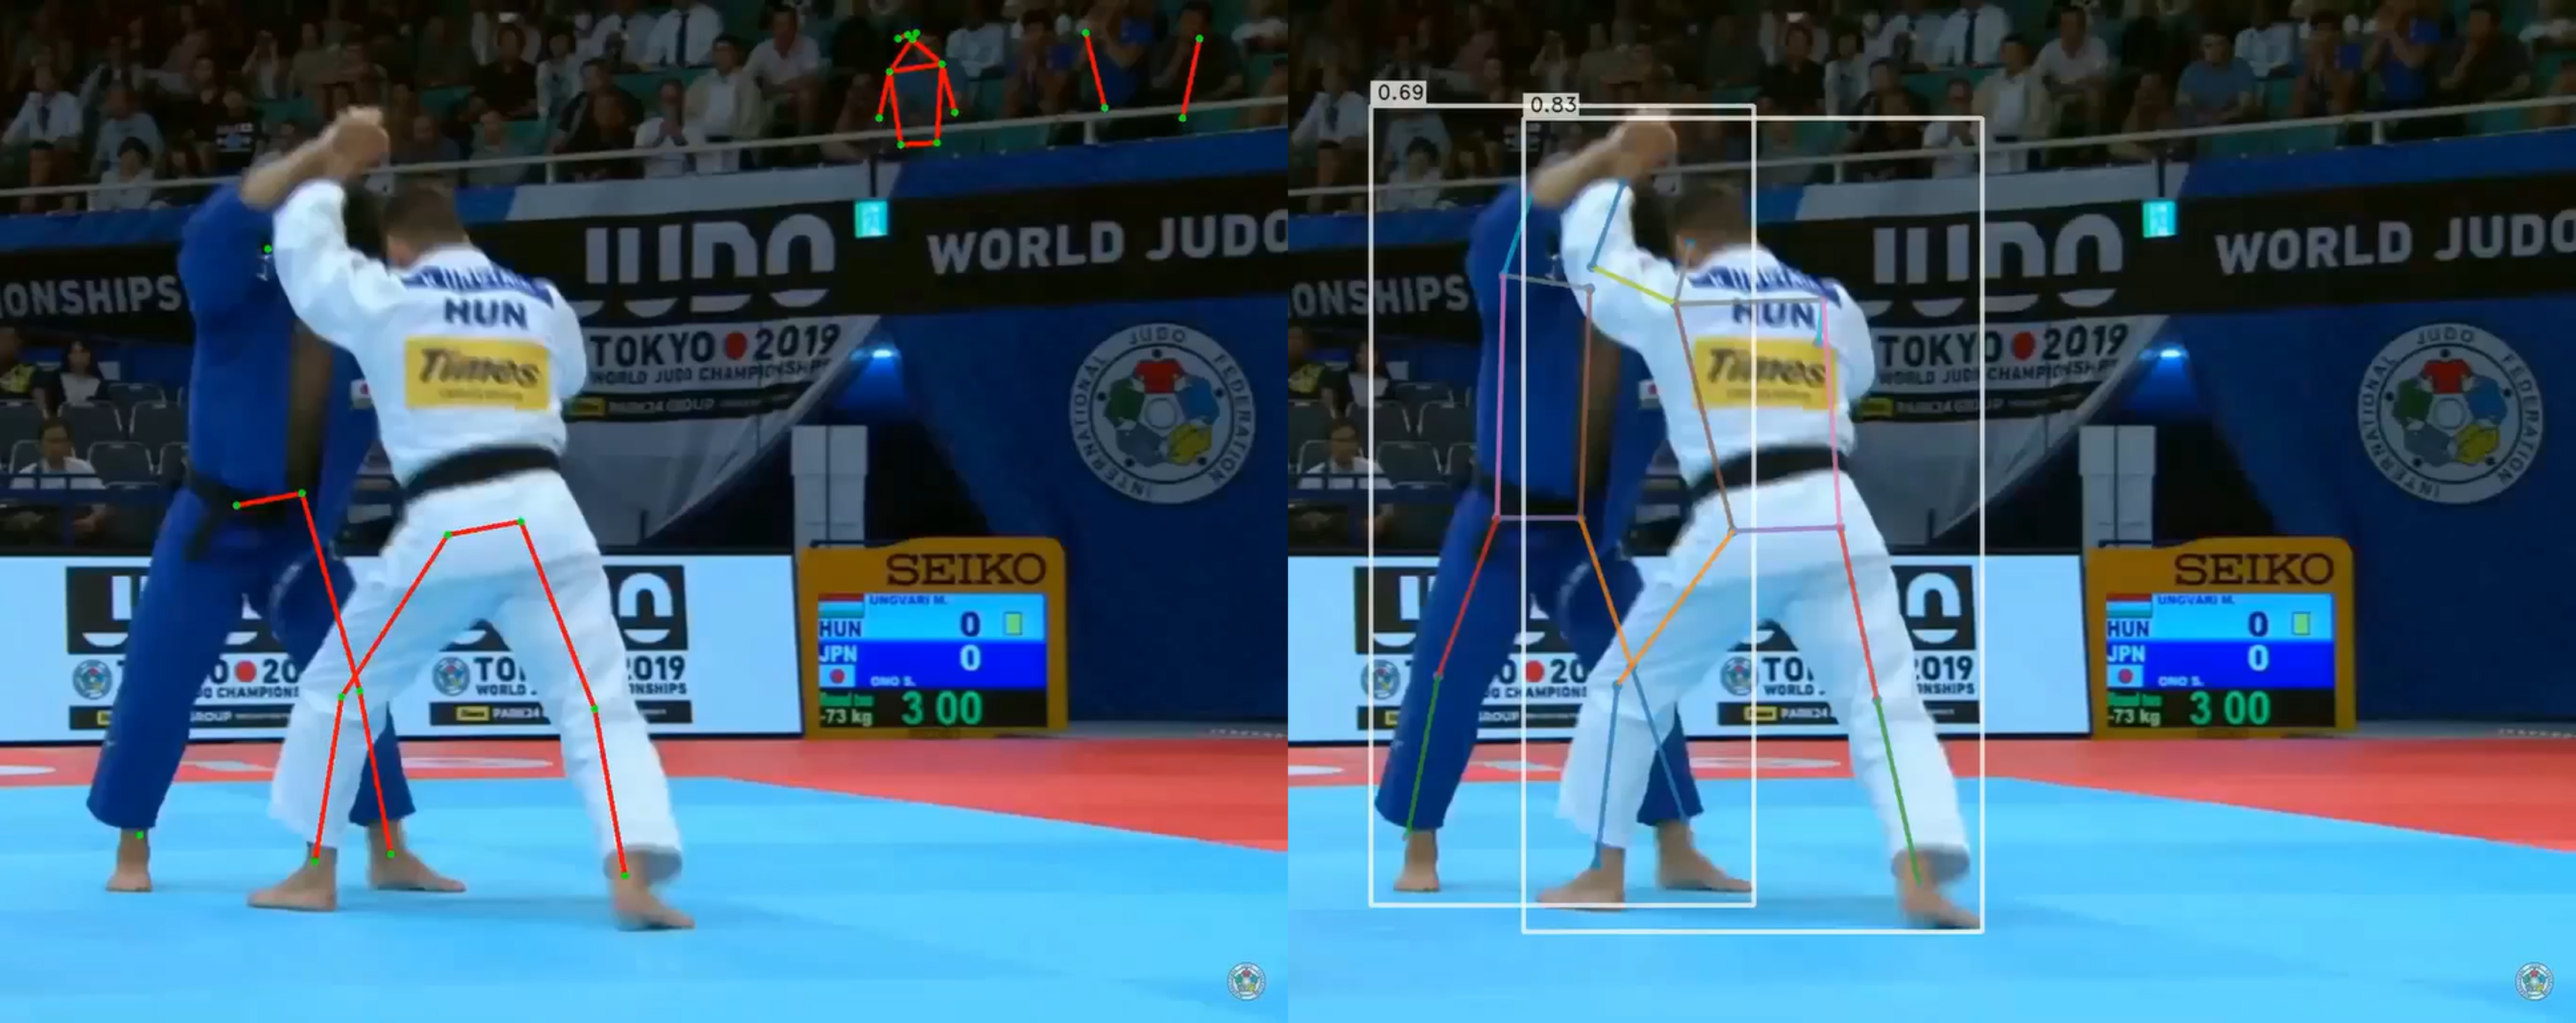
\includegraphics[scale = 0.5]{img/MoveNetvsYOLO.png}
    \caption{A comparison of MoveNet Lightning (left) and YOLO-NAS-POSE-L (right).}
    \label{fig:comparingHPEmodels}
\end{figure}

\bigskip
\noindent
YOLO-NAS-POSE also allowed for individual frame processing, batch frame processing or direct video processing, and supported both live capture/playback and file-based I/O. 

\bigskip
\noindent
YOLO-NAS-POSE is available in 4 variants - N, S, M and L. The previous comparison made use of YOLO-NAS-POSE-L, the highest accuracy model available from Deci AI. The table below is sourced from Deci AI's documentation - AP numbers in table reported for COCO 2017 Val dataset and latency benchmarked for 640$\times$640 images on Nvidia T4 GPU. No flip-TTA was used. \cite{DeciAI}

\bigskip
\begin{center}
\begin{tabular}{|c c c|} 
 \hline
 \textbf{Model} & \textbf{AP (Accuracy)} & \textbf{Latency (ms)} \\ [0.5ex] 
 \hline
 YOLO-NAS N & 59.68 & 2.35 \\ 
 \hline
 YOLO-NAS S & 64.15 & 3.29 \\
 \hline
 YOLO-NAS M & 67.87 & 6.87 \\
 \hline
 YOLO-NAS L & 68.24 & 8.86 \\ 
 \hline
\end{tabular}
\end{center}

\begin{figure}[ht]
    \centering
    \includegraphics[scale = 0.35]{img/yolo_nas_pose_l.png}
    \caption{A comparison of various HPE models by Deci AI. \cite{DeciAI}}
    \label{fig:comparingYOLOModels}
\end{figure}

\bigskip
\noindent
I opted to use YOLO-NAS-POSE-L for the project, because of its superior accuracy compared to other variants.


\subsection{The Classifier}

Most other solutions in the field of object/action recognition and classification make use of deep convolutional neural networks (DCNNs) \cite{DCNN}. However, DCNNs will not be used for this project, because they train slowly, require a massive amount of data, and require very powerful hardware \cite{DCNNDisadvantages}. While DCNNs may provide great performance benefits, the trade-off is too large for them to be considered a viable solution - a sufficiently large dataset is not available at this time and cannot be easily generated and labelled. Additionally, one of the key benefits of DCNNs, feature extraction, is performed earlier in the pipeline, by the human pose estimation model, which extracts the keypoints of the athletes through computer vision techniques.

\bigskip
\noindent
Instead, a neural network with three layers will be used (multi-layered perceptron). Neural networks can be used to perform binary classification by having an output layer of a single sigmoid-activation neuron. This architecture was chosen based off of the research conducted by V. Hudovernik et al., who used a multi-layered perceptron with an input layer of 102 neurons, a hidden layer of 34 neurons and an output layer of 18 neurons (corresponding to 18 possible classes) \cite{IdentifyingBJJPositions}. 102 input neurons is a necessity, because the pose estimation model outputs 17 keypoints for 2 people, each keypoint of the form $(x, y,  \textit{confidence})$, and $17 \times 2 \times 3 = 102$ input neurons. For the output layer, as aforementioned, will have a single neuron. The hidden layer will consist of 34 neurons, drawing inspiration from the architecture outlined by V. Hudovernik et al \cite{IdentifyingBJJPositions}. A benefit of using a simpler MLP over a large DCNN is that training will be much faster, even on weaker hardware, and the resultant model will be much more portable. 

\begin{figure}[ht]
    \centering
    \includegraphics[scale = 0.25]{img/MLP.drawio.png}
    \caption{MLP model for classification.}
    \label{fig:MLPdiagram}
\end{figure}

\bigskip
\noindent
The MLP will use binary cross-entropy loss, as this loss function is used heavily in conjunction with binary classification problems \cite{BinaryCrossEntropyLoss}. The Adam optimization algorithm will also be used, as it has seen an increase in use for computer vision over the last few years \cite{AdamOptimiser}. As mentioned previously, the output layer will use the sigmoid activation function, as it outputs values between 0 and 1. These values can be interpreted as probabilities, where values closer to 1 indicate "pin", and values closer to 0 indicate "no pin". This also makes training very simple, as the dataset has been adapted to contain labels that are either 1's or 0's for every datapoint. The input and hidden layer neurons will use ReLU (rectified linear unit) as their activation function. ReLU computes much faster than the sigmoid function, allowing for faster training times.

\bigskip
\noindent
The classification machine learning algorithm will be created using PyTorch, a popular and well-documented Python library for machine learning. PyTorch is a library that is familiar and compatible with other elements of the project, making it an ideal choice. PyTorch also allows for models to be saved and loaded as files, adding a degree of modularity and portability to the project.

\section{Implementation}

The implementation stage of the project is divided into three key areas:
\begin{itemize}
    \item The HPE model
    \item The MLP classifier
    \item Image and video handling
\end{itemize}

Please note - development did not follow this sequence strictly throughout implementation.

\subsection{The HPE Model}

\subsubsection{Assessing HPE Models}

\noindent
As mentioned previously, three pre-trained HPE models were selected and evaluated for their suitability for the problem, before the main implementation began.

\bigskip
\noindent
The first model to be assessed was MediaPipe Pose Landmarker. I implemented a minimal version on a Jupyter Notebook, hosted by Google Colab. While promising and fairly accurate, it was notably slow, especially when using live video feed. It was at this point that I made the decision to use secondary storage as the primary means of communicating with the user, rather than real-time recording and playback. Additionally, MediaPipe seemed to suffer a dramatic drop in performance when occlusion was involved - if I concealed a limb such that it could no longer be seen by my webcam, and then brought it back into view, the model would struggle to register it again. The largest issue, however, was that the keypoint locations did not match that of the dataset, making this model infeasible for this project. In the figure below, there is a kinematic model of myself on the far left, experimenting with MediaPipe through my webcam.

\bigskip
\begin{figure}[ht]
    \centering
    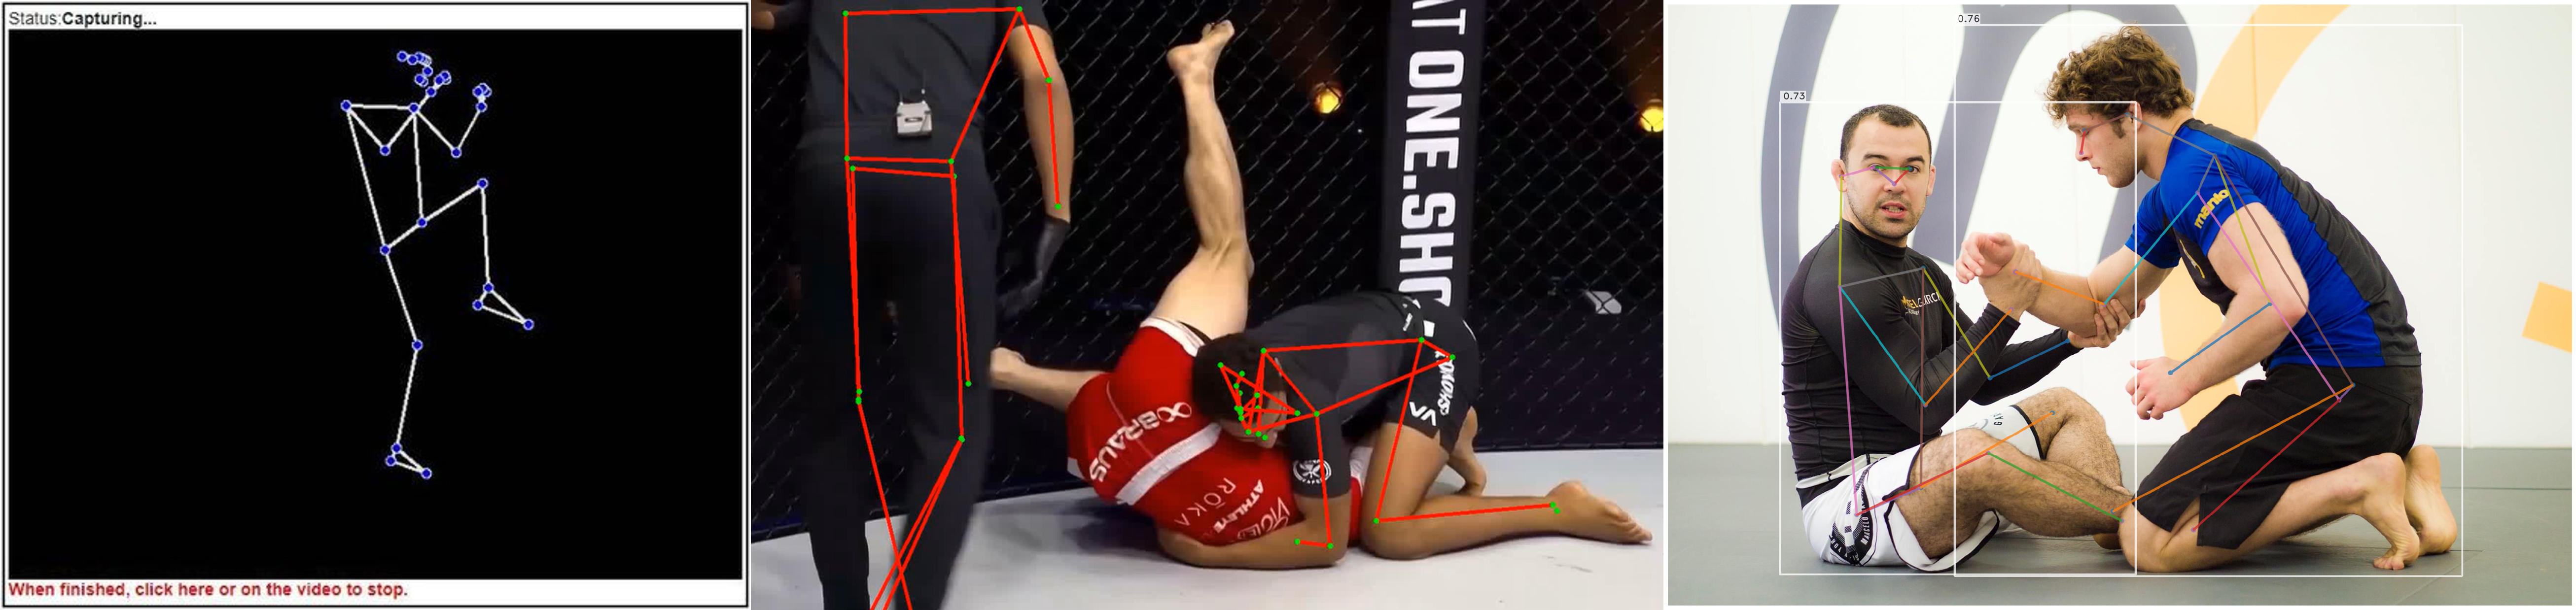
\includegraphics[scale = 0.42]{img/themodels.png}
    \caption{From left to right: MediaPipe, MoveNet Lightning, YOLO-NAS-POSE-L.}
    \label{fig:assessing-models}
\end{figure}

\bigskip
\noindent
The next model evaluated was MoveNet Lightning. Once again, I implemented a minimal version using Google Colab. MoveNet Lightning was extremely promising - fast, accurate and customisable, however issues arose when I sampled videos of people moving quickly. MoveNet seemed to struggle to keep up with multiple individuals, and the performance dropped even more when competitors were on the ground. Additionally, MoveNet would pass back video files with a much lower frame-rate compared to the original inputs. Considering that much of grappling encompasses ground-fighting, MoveNet was not an option viable option for this project. In the above figure, middle, there is a snapshot of a single frame from a professional Jiu-Jitsu match.

\bigskip
\noindent
YOLO-NAS-POSE (large variant) was the final model assessed. This model was assessed using a Jupyter Notebook released by Deci AI, designed to showcase the model in action. Immediately, the adjustable confidence level made this model an appealing solution, as with grappling, a lower confidence level may be better - it allows models to output hypothesised keypoint locations that it may not have been confident with otherwise. YOLO-NAS-POSE-L was consistenly the fastest model tested thusfar, easily processing images within 4-5 secs, even without a GPU. The model performed well on images and video alike, and the provided \texttt{predict()} function handled both video and image input natively. Above, far right, is an example of the model in action with two Jiu-Jitsu practitioners. In the example, the model successfully predicts almost all keypoints of either competitor, despite both of them being in close proximity and on the ground.

\subsubsection{YOLO-NAS-POSE}

The \texttt{supergradients} library was installed to enable loading of the the YOLO-NAS-POSE-L model. Firstly, a wrapper function for the aforementioned \texttt{predict()} function was written, called 

\noindent
\texttt{predict\_image()}. This wrapper was written to handle the input path of the location of the image, or an image represented by a \texttt{numpy} array. The model returns an \texttt{ImagePoseEstimationPrediction} object, which is contains the keypoints of the competitors in its \texttt{poses} attribute. The default confidence (acceptance threshold for outputting a pose candidate) was set to 0.3. This was done after experimentation with different confidence levels, and is explained and justified in the next section.

\bigskip
\noindent
The \texttt{extract\_poses()} method takes an \texttt{ImagePoseEstimationPrediction} object, accesses its \texttt{poses} attribute to obtain the keypoints, and reformats the keypoint arrays to a single \texttt{numpy} array with a length of 102. This reformatting allows the data extracted from the object to easily be passed to the MLP for classification. The remaining HPE model-related functions and methods are integrated with the image and video handling methods. As such, they are included in the third subsection.

\subsection{The Classifier}

\subsubsection{Data Parser}

Before implementing the classifier, data had to be loaded and parsed from the CSV file, to enable training and testing. A function \texttt{init\_data()} was implemented to parse a given CSV file using the \texttt{pandas} library. Data needed to be parsed before training to allow the dataset to be split into train and test sets, and other data operations.

\bigskip
\noindent
The labels were extracted from the dataset, and placed in \texttt{numpy} arrays. However, the features were stored in the CSV file as strings, and under two fields - "pose2" and "pose1". In order to be suitable for training, features needed to be stored with all coordinates and confidences for both combatants stored in a 1-D array of length 102. This was done using the \texttt{ast} library to evaluate the strings as lists, before converting them to \texttt{numpy} arrays and flattening them.

\bigskip
\noindent
At this point, there were two key data structures - \texttt{X}, a matrix containing the features, where rows a single row in the matrix corresponds with a single row of the dataset, and \texttt{y}, an array of the corresponding labels. Normalisation was carried out on \texttt{X}, but not \texttt{y}, since \texttt{y} was already normalised, containing only 0's and 1's. \texttt{X} and \texttt{y} were split into train and test sets, with 20\% of data going into the test set, and the rest going into training. This split was chosen because the task at hand requires a large amount of training data, and this is the general practice when working with machine learning.

\bigskip
\noindent
After splitting the data into train and test sets, each individual set had random oversampling applied to them, using the \texttt{imblearn} library \cite{imbalancedlearn}, in order to achieve a perfect 50:50 split of the binary classes (pin and no-pin). Random oversampling was performed after the \texttt{train\_test\_split()} in order to prevent data from duplicating across the split datasets, which may have resulted in holdout set leaking into the training set, which would likely lead to overfitting and hence an inaccurate assessment of the model later on, during the testing phase. 

\subsubsection{Implementing the MLP}

The \texttt{torch} library was installed to enable the creation and training of the multi-layered perceptron. An \texttt{MLP} class was implemented (as specified previously), as well as a wrapper function for making predictions using the MLP class (called \texttt{predict\_position()}). A wrapper function was used because we want to control what data gets sent to the MLP. In the case that there is an array of only 51 values (as opposed the expected 102) sent to the MLP, we want to reject this, as it may lead to unexpected results or outputs from the MLP.

\bigskip
\noindent
A case where an array of unexpected length (such as 51) may be sent to the MLP is in the case that the HPE model can only detect one person. Because we know that an individual cannot technically pin themselves, we know for sure that a pin will not be detectable on the screen. In this case, we simply return a float value of 0.0, indicating that there is not a pin detectable in the original input image. Similarly, if there is a case where there is more than 102 inputs received (i.e. there are more than 2 people present in the given  image), we also return 0.0, as handling images with more than two people falls outside of the scope of this project.

\bigskip
\noindent
The functions \texttt{save\_model()} and \texttt{load\_model()} were also created, to provide a fast and safe way to save and load the state dictionary of the MLP to the file-system as a \texttt{.pt} file. 

\bigskip
\noindent
Finally, the functions \texttt{train\_model()} and \texttt{test\_model()} were written, to train and test the model on a given dataset. In \texttt{train\_model()}, the model is trained for a given number of epochs, and the loss (error) for every epoch is displayed. All losses are also stored in an array, which is returned by the function. This can be used for analysis or improvement of the model in the future, as well as for visualising data. \texttt{test\_model()} evaluates the model's performance on every item in the holdout set, keeping track of correct and incorrect answers, and outputting it at the end, to allow evaluation of the MLP. 

\bigskip
\noindent
The MLP was trained and evaluated over 25, 50, 100, 200, 500 and 1000 epochs. The errors over the training periods are shown below.

\bigskip
\begin{figure}[ht]
    \centering
    \includegraphics[scale = 0.59]{img/all_epochs.png}
    \caption{Graphs showing error of classification model over different epoch ranges. Top row, left to right: 25 epochs, 50 epochs, 100 epochs; bottom row, left to right: 200 epochs, 500 epochs, 1000 epochs.}
    \label{fig:all_epochs}
\end{figure}

\bigskip
\noindent
(The resultant test result scores are shown and discussed in-depth in the next section.)

\bigskip
\noindent
Even after training for 1'000 epochs, the model still showed a steady downward trend in loss (despite some spikes), and an increase in accuracy on the test (holdout) dataset. As a result, even with it's apparent that even after 1000 epochs of training, overfitting hasn't become an issue yet. As a result, the saved (supplied) model will be one which has been trained for 1'000 epochs, due to superior performance.

\subsection{Image and Video Handling}

The aptly named functions \texttt{split\_video\_into\_frames()} and \texttt{concat\_frames\_into\_video()} are designed to work such that the frames extracted from the video can be treated as independent images, and processed by the pose estimation model and classifier as shown below. They make use of the \texttt{cv2} library.

\bigskip
\begin{figure}[ht]
    \centering
    \includegraphics[scale = 0.23]{img/video-processing-pipeline.drawio.png}
    \caption{A simplified image and video processing pipeline.}
    \label{fig:image-video-pipeline}
\end{figure}

\bigskip
\noindent
\texttt{split\_video\_into\_frames()} returns a list of frames (images), and each frame in this list is passed to the machine learning models for processing. When these models are done, they pass a new frame back in response, with the appropriate annotations and predictions made. All of these frames for a video are then aggregated and passed to \texttt{concat\_frames\_into\_video()}, which creates a new, annotated video and saves it to the file-system. The framerate of the original video is retained in the variable \texttt{fps}, to ensure that the returned video is exactly the same speed as the original. I also implemented \texttt{save\_image()}, a function that uses \texttt{cv2} to save an image to a given path.

\bigskip
\noindent
Following on from the implementation of the HPE model and its associated functions, I implemented a group of functions to annotate the image according to the output of both the HPE model and the classifier. Before doing this, I needed to determine the colour of the annotations - as mentioned earlier, the annotation colour is green if the classifier believes a pin is present in the image (i.e. when the MLP returns a value greater than 0.5), or red if the classifier believes otherwise. The function \texttt{predict\_text\_color()} implements this logic, by taking the prediction of the MLP, and returning the appropriate text and colour.

\bigskip
\noindent
The \texttt{supergradients} library provides a \texttt{save()} method for the \texttt{ImagePoseEstimationPrediction} class, used for drawing keypoint and edge annotations to an image, and saving the image. However, I discovered a bug in the source code that prevented custom colours from being used in the image as intended. I have opened a pull request on GitHub and the issue is ongoing - as a result, I have implemented my own \texttt{draw\_keypoints()} method, which takes a \texttt{ImagePoseEstimationPrediction} object and a desired colour, and returns a new image as a \texttt{numpy} array, with the keypoints and edges drawn over the original image.

\bigskip
\noindent
\texttt{annotate\_image()} behaves similarly to \texttt{draw\_keypoints}, except that it takes an image (as a \texttt{numpy} array), a float result from the MLP classifier (confidence), the text to be written and the colour to use (both based on the classification made by the MLP). This function uses \texttt{cv2} to write to the image, and returns the modified image. At this stage, the image returned here is to be passed back to the user, by saving it to the file-system.

\bigskip
\begin{figure}[ht]
    \centering
    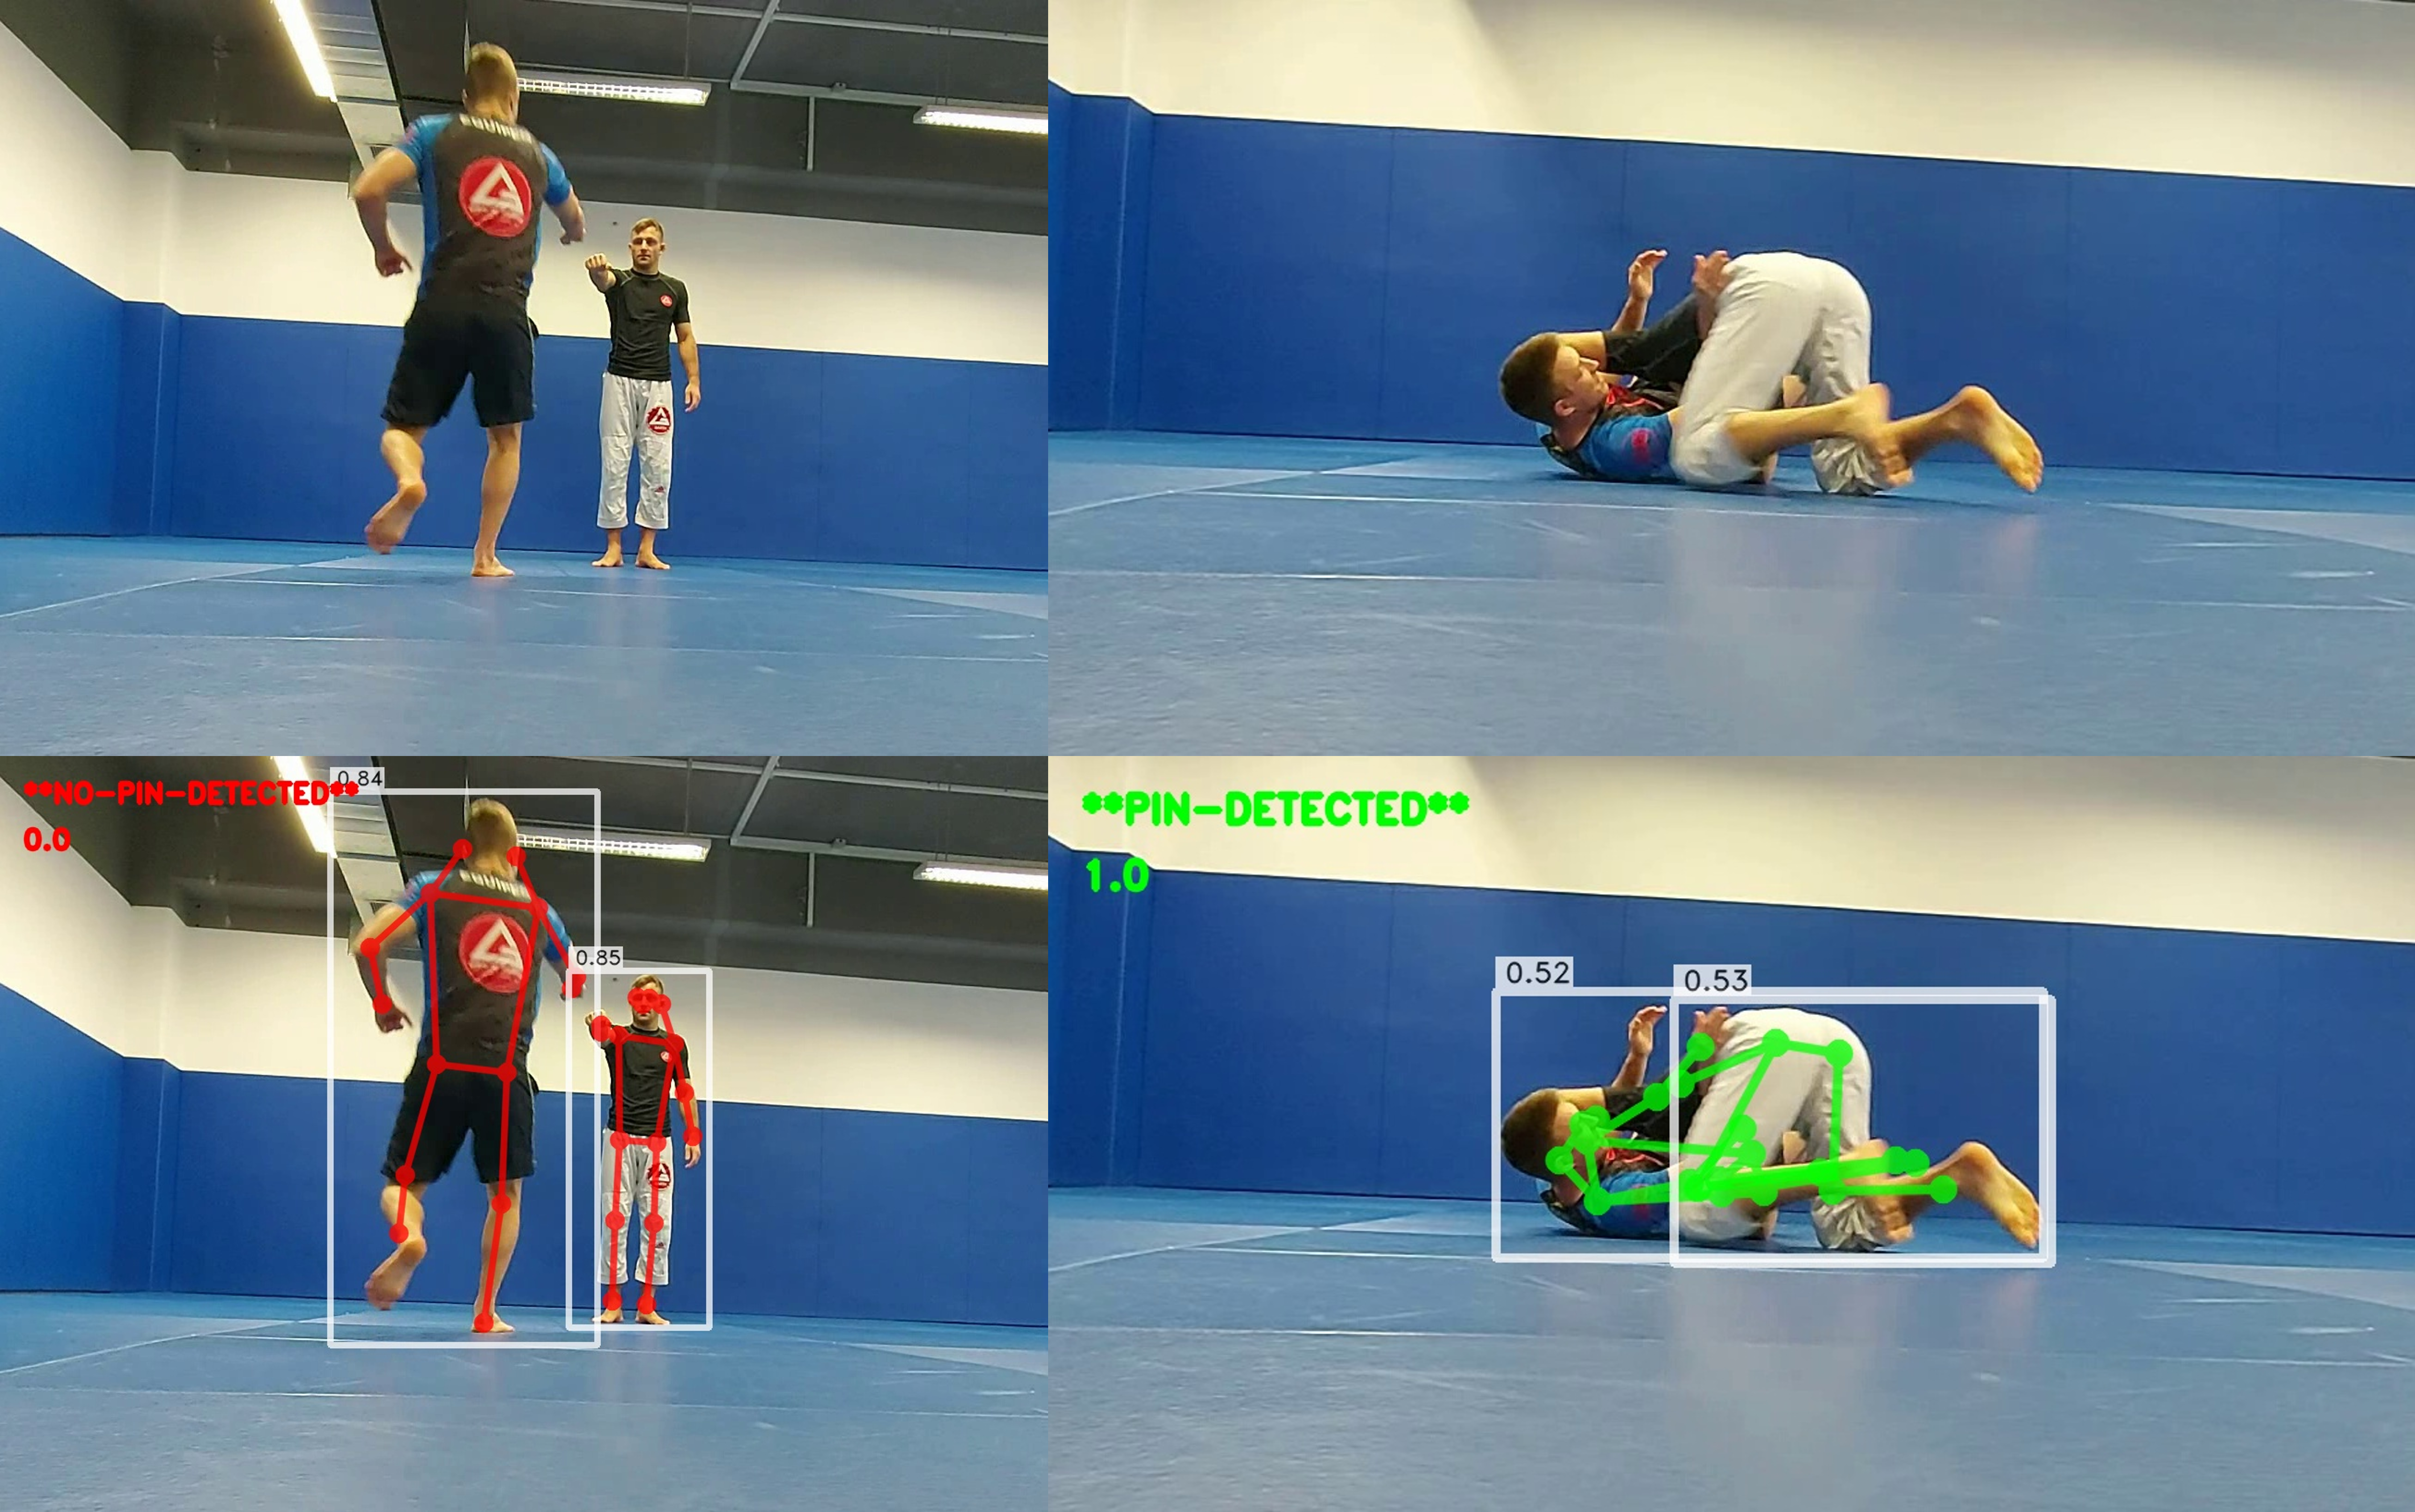
\includegraphics[scale = 0.435]{img/working_examples.png}
    \caption{Two examples of the full pipeline in effect. The top row contains two original images from the dataset, and the bottom row shows the output when these images are passed through the pipeline.}
    \label{fig:working-examples}
\end{figure}


\newpage
\bigskip
\section{Testing}

\subsection{The Classifier}

As mentioned in the previous section, the classifier was trained and tested over a variety of epochs. In the previous section, we saw many graphs of the error level over the epochs. On all iterations of the model, loss trended downwards as training continued. However, on some of the models (especially those training over more epochs), there were sudden strange spikes in error during training. At first, I was concerned that this may be indicative of overtraining or some other issue, but after performing some research, I determined that as long as the loss continues to trend downwards, and test score improves, these loss spikes aren't of any concern.

\bigskip
\noindent
In order to keep time durations fair and runs independent, on each run (with a new number of epochs), the model was made to reload data from the CSV and reinstantiate itself. The times shown below are the times taken for the model to load the data, instantiate, train (for some number of epochs) and test. The results shown below are the scores of different runs on the test dataset of 25'163 datapoints. For consistency, all of these runs took place on the same Google Colab runtime, CPU only. 

\bigskip
\begin{center}
\begin{tabular}{|c c c c|} 
 \hline
 \textbf{Epochs}   & \textbf{Correct (out of 25163)}  & \textbf{Accuracy (\%) } & \textbf{Time taken (s)} \\ [0.5ex] 
 \hline
 25 & 20219 & 80.35 & 40 \\ 
 \hline
 50 & 20615 & 81.93 & 48 \\
 \hline
 100 & 21069 & 83.73 & 47 \\
 \hline
 200 & 21318 & 84.72 & 58 \\ 
 \hline
 500 & 22265 & 88.48 & 86 \\ 
 \hline
 1000 & 23366 & 92.86 & 134 \\ 
 \hline
\end{tabular}
\end{center}

\bigskip
\noindent
With the above, we can see that the even as epochs increase, the score on unseen data continues to improve. These runs were repeated several times with the same epoch counts, and at 1'000 epochs, the classifier consistently achieves 90\%+ accuracy on unseen data, which is considered very, very high in a problem like this.

\bigskip
\noindent
A confusion matrix was also generated for the 1000-epoch model, after several more test runs, shown below. This confusion matrix was generated from the holdout (test) dataset.

\bigskip
\begin{figure}[ht]
    \centering
    \includegraphics[scale = 0.8]{img/confusion_matrix.png}
    \caption{Two examples of the full pipeline in effect. The top row contains two original images from the dataset, and the bottom row shows the output when these images are passed through the pipeline.}
    \label{fig:confusion-matrix}
\end{figure}

\bigskip
\noindent
We can see that the 1000-epoch model has fairly accurate predictions for both labels, and there are no massive outliers in type I or type II errors. The result is an extremely strong and successful classifier, that works effectively on unseen data despite having a relatively simple architecture.

\bigskip
\noindent
Using the confusion matrix, we can calculate the F1-score of the classifier. 
\begin{itemize}
    \item Precision = $\frac{TP}{TP + FP} = \frac{10876}{10876+1672} = \frac{2719}{3137} = 0.87$
    \item Recall = $\frac{TP}{TP + FN} = \frac{10876}{10876+1706} = \frac{5438}{6291} = 0.86$
    \item Accuracy = $\frac{TP + TN}{TP + FP + FN + TN} = \frac{10876 + 10910}{10876 + 1672 + 1706 + 10910} = \frac{3631}{4194} = 0.87$
    \item F1-score = $2 \times \frac{Precision \times Recall}{Precision + Recall} = 0.87$
\end{itemize}

With an F1-Score of 0.87, the classifier can be considered a success. However, it's worth noting that the model may not perform as well on other datasets - this is discussed further in the next section.

\subsection{End-to-End Testing}
During implementation, continuous informal end-to-end tests were carried out, aiming to approximately optimise the confidence (acceptance) threshold for the HPE model. Eventually, an acceptance level of 0.3 was chosen, as this seemed to yield the best chance at detecting both players when they are engaged in combat. While 0.3 is a very high acceptance level for other HPE applications, in this case, it's quite acceptable - other HPE applications rarely have to deal with as high a level of occlusion, and this level of acceptance allows the model more opportunity to detect an athlete in a more complicated position.

\bigskip
\noindent
Unfortunately, due to the nature of the computer vision model, there are no easy or conventional tests available - the model makes use of pre-trained weights, and training methods are largely informal, non-automated and arduous. Nevertheless, some attempt has been made to evaluate the performance of the HPE model, through end-to-end testing (i.e. using the final product).

\bigskip
\noindent
I performed back-to-back end-to-end tests on a random subset of the original dataset, consisting of 1'000 images, and visually analysed the outcome. The performance of the overall product was strongly bottlenecked by the shortcomings and limitations of the HPE model. Unfortunately, during the most occluded combat scenes, the model could only make out one of the two combatants on-screen at a time. Despite experimenting with confidence thresholds, there were times during the exchange that one athlete was simply barely visible, with all of their body being covered by the opposing athlete. In such cases, since only one person was visible in the frame, the program would default to "NO-PIN", as per the logic implemented earlier, where if the number of people present is not equal to 2, a pin cannot take place.

\bigskip
\begin{figure}[ht]
    \centering
    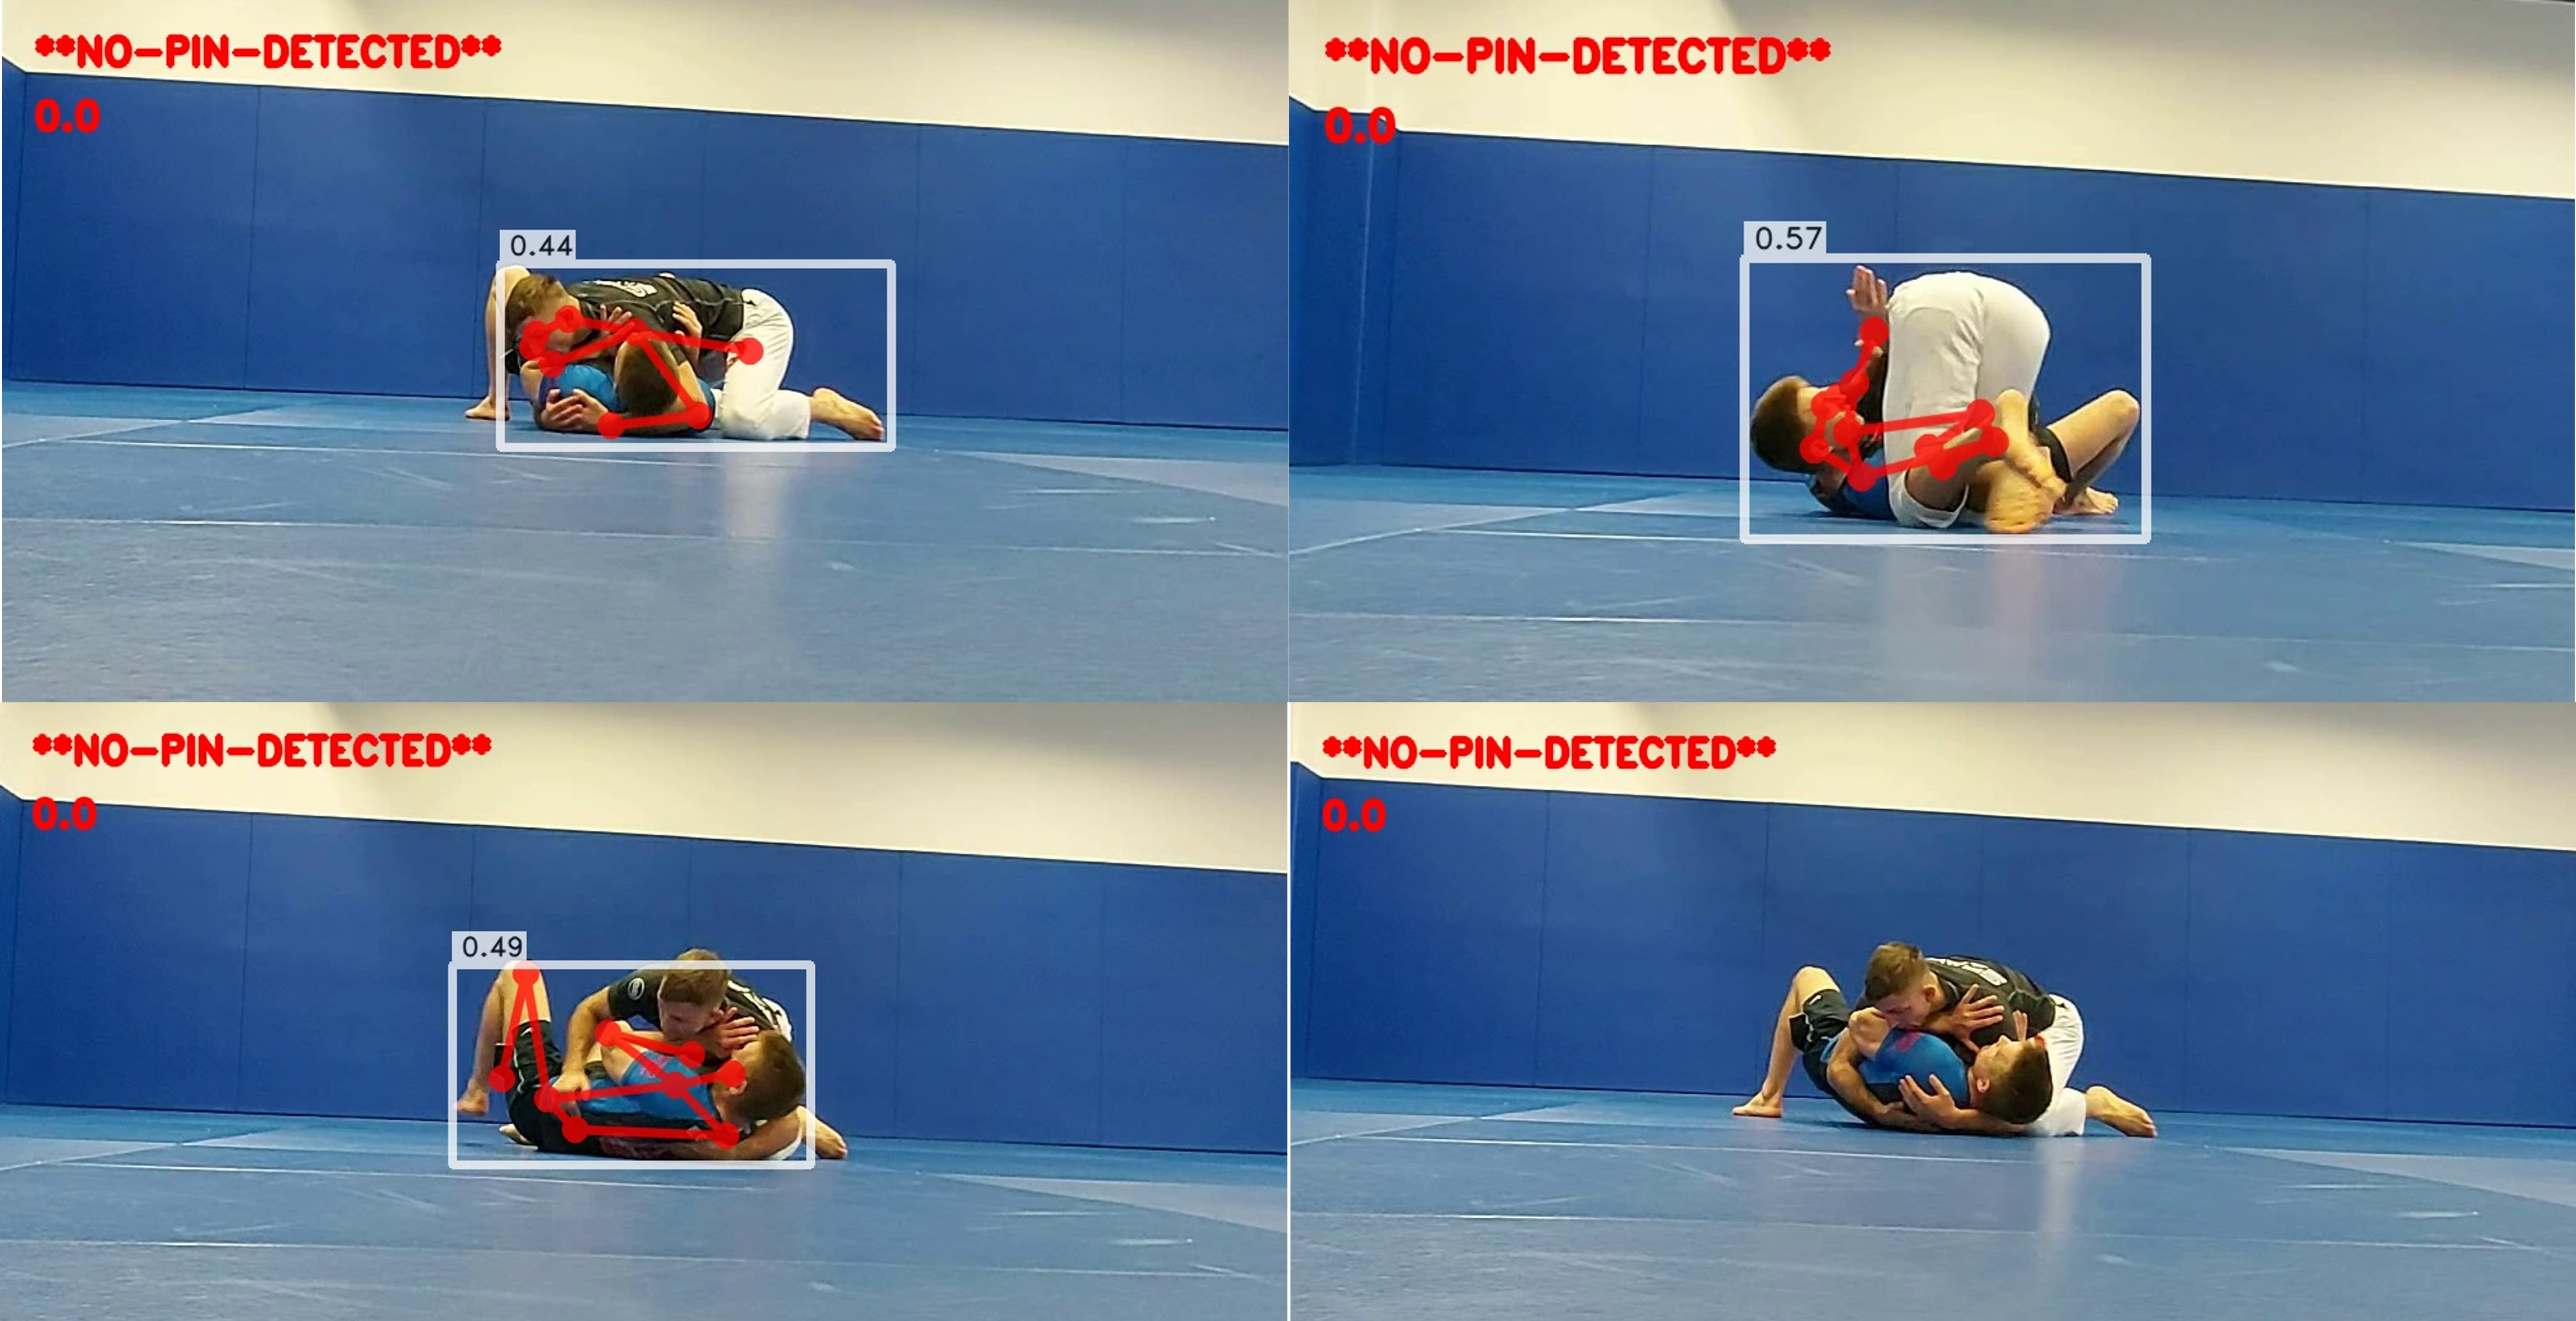
\includegraphics[scale = 0.52]{img/fails.png}
    \caption{Four examples of the HPE model failing to recognise both athletes, resulting in the classification being wrongly predicted.}
    \label{fig:fails}
\end{figure}

\bigskip
\noindent
In the figure above, one combatant has the other pinned in side control in all four images. However, the HPE model fails to detect both athletes in all images - in fact, on the bottom right image, the model fails to detect anyone. This demonstrates how failure on the part of the computer vision model impacts the entire pipeline, and always results in an incorrect output. This will be discussed further in the next section. 

\bigskip
\noindent
Regardless of the issues with outcomes, the pipeline is highly efficient even on weaker hardware, and a full pipeline execution for a single image can be completed on CPU in typically under 5 seconds.

\subsection{Performance on Video}

\noindent
Because video input is treated as a series of frames (images), the performance on videos (in terms of accuracy) will be identical to that of images. This means that video inputs have the same high classification accuracy (when both athletes are correctly detected), but suffer from the same issues when it comes to detecting and identifying the keypoints of each athlete.

\bigskip
\noindent
However, in terms of speed, there is a lot of variation. The speed of video processing is largely dependent on the framerate of the input video - a video captured at 60 frames per second will, on average, process twice as slow as a video captured at 30 frames per second (ignoring overhead from dissecting and restitching video).

\bigskip
\noindent
When compared to YOLO-NAS-POSE-L's native video processing support, or batch image processing, the product is signficantly slower. Without GPU support, even a short video clip can take a relatively long time to process through the pipeline, and we can infer that much of this is due to the inefficiency of serially processing video frames, since we know that the binary classifier introduces barely any overhead, and that image processing on a single image, even on CPU, is quite fast and efficient. This will be discussed further in the next section.

\section{Evaluation and Critical Assessment}
\subsection{Description of the Final Product}

The final product is a series of functions in a Jupyter Notebook that allow a user to take an image or video file from their local directory, load it, process it through a computer vision model for detecting human beings and their keypoints (joints), use these keypoints to determine whether or not a grappler has successfully pinned another grappler (in the image/video), modify the image/video to reflect this prediction, and output the image/video to the user's file-system.

\bigskip
\noindent
The final product also provides a data parser, which parses data from an appropriately formatted CSV file, and multi-layered perceptron class for binary classification, which can be instantiated, trained on some parsed data, and evaluated on some holdout test data. The metrics and performance of this classifier are then displayed. Customisable arguments are provided to change the behaviour of the training and test phases, such as modifying the data split and changing the number of epochs trained for.

\subsection{Successes}

Evaluating against the success criteria, the project enjoys a favourable result. Criteria 1a and 1b are a success - the program handles video as expected, splitting them into frames and rejoining them into a video at the end of the pipeline. Similarly, the features outlined by criteria 2a-2e are all present and implemented successfully. 3a is a success, however, 3b is not - video processing takes too long and scales fairly poorly. 4a is a partial success - a HPE model has been used, but it was not entirely implemented independently, instead, using pre-trained weights. 4b is a full success. The fifth criteria is overwhelmingly successful; the final F1-score on an unseen dataset by the classifier (with 1'000 epochs of training) was 0.87, much larger than the minimum of 0.7. Finally 6a-6c is fairly successful, as methods have been provided to save and load machine learning models, as well as this report, which outlines in detail the steps taken during implementation and how one may recreate the results.

\bigskip
\noindent
However, reflecting upon the success criteria themselves, I do strongly feel like they could've been much more encompassing with regards to performance and practicality. In the future, I would look to outline success criteria that take a more wide range of factors into account, and use more metrics to measure the project success. Going outside of the success criteria, by far the largest success of the project is that of the classifier. The idea of performing feature extraction through a pose estimation model prior to classification proved to be a great one, as it provided a much simpler, more portable and faster to train on alternative to contemporary deep convolutional neural networks. 

\subsection{Limitations}

By far the most damning limitation of the project is the inability to work when there are less than or more than two people in an image. This is a severe issue because, when in conjunction with an occluded image where only one athlete is visible, the program automatically assumes that a pin cannot be present. While this is true technically, perhaps it would've been wiser to not immediately declare that there is no pin present, but rather to analyse the visible individual, and make inferences based on their anatomical position. This is discussed further in the next section. 

\bigskip
\noindent
Another limitation of the project is that it most likely isn't ready for real-world applications. I occasionally ran grappling images through the pipeline that were not from the dataset, and the program consistently provided incorrect outputs. There are many factors simply are not accounted for in this project, that have a very real impact on the performance of a computer vision model. Lighting, camera angles, moving cameras and zoom are all factors when it comes to recording real grappling exchanges, and the project simply is not built to reckon with any of these issues.

\subsection{Outlook and Potential Future Work}

While some aspects of the project were highly successful, other aspects and ideas could have been improved. The largest issues and bottleneck came from failure on the part of the HPE model, and unfortunately there's very little that can be done about this - HPE in occluded environments is a problem that no viable solutions exist for at this time. Nonetheless, the work done on this project can very easily be used in future projects, as the proposed pipeline is easily applicable to a variety of sports, even outside of combat sports. 

\bigskip
\noindent
Developing a pose estimation model that is capable of filtering out unwanted individuals in a scenario would be a huge benefit to this project, as it would allow for much better potential real-world performance. One of the biggest factors hampering the pipeline from working in a practical scenario is the inability to deal with additional people, besides the two combatants. This is an issue because in a live grappling match, there may be an audience, a referee, judges and other characters who are more than likely to appear in-frame, along with our competitors. Being able to filter them out, or discard their keypoints would prove very useful. One way the latter could potentially be done is through measuring Euclidean distance between keypoint groupings, and identifying which pair of groupings are likely to belong to both athletes. This task of distinguishing the athletes from everyone else would likely be assigned to a machine learning algorithm, and would prove a valuable addition to the existing pipeline, intersecting between the HPE model and the classifier. 

\bigskip
\noindent
As mentioned in the previous section, the idea to assume that a pin cannot be present when there's only one individual present, while seemingly logical, places an unrealistic amount of dependence on the capabilities of the HPE model. For a future project, it may be wiser to still analyse the position of an individual athlete (when they are the only person visible), and consider if it's probable that they are concealing the other athlete with their body. Again, this would add another module to the pipeline, but drastically improve performance when working with awkward angles and positions. Finally, in order for the model to be successful in the real world, a significantly larger dataset is likely needed, and perhaps more computational power to handle the increased load. Convolution could be employed to further distinguish details of positions and provide additional insight and nuance into grappling.

\bigskip
\noindent

\section{Conclusion}

The aim of this project has been to create a system to identify the presence of a pin in a grappling exchange between two combatants, through the use of computer vision and binary classification. A system has been developed that takes input from image or video, and outputs a modified version of the input image, where keypoints are drawn on either athlete, and an annotation is added to indicate whether or not a pin is present in the image.

\bigskip
\noindent
The project has been moderately successful, and while not all aspects of the final product operate as well as intended, the project itself presents a framework upon which future projects may base themselves, by using the pipeline of a human pose estimation algorithm and a machine learning classifier. Future projects can use the ideas presented here for similar applications with any sport where position is a key factor to winning a match.


\newpage
\pagenumbering{roman}

\printbibliography

\end{document}